\documentclass[a4paper,12pt,twoside]{article}
\usepackage[utf8]{inputenc}
\usepackage[italian]{babel}
\usepackage{bigints}
\usepackage{graphicx}
\usepackage{geometry} 
\usepackage{float}
\usepackage{url}
\usepackage{xcolor}
\usepackage{enumitem}
\geometry{a4paper,top=3cm,bottom=3cm,left=3cm,right=3cm}
\linespread{1.5}
\graphicspath{ {./Images/} }
\usepackage{setspace}
\usepackage{listings}
%% Package Numerazione
\usepackage{fancyhdr}
\fancyhf{} % clear all header and footers
\renewcommand{\headrulewidth}{0pt} % remove the header rule
\fancyfoot[LE,RO]{\thepage} % Left side on Even pages; Right side on Odd pages
\setlength\parindent{24pt} % PER INDENTARE
%\hspace{\parindent} % DA METTERE NEI SINGOLI PARAGRAFI
\pagestyle{fancy}
\fancypagestyle{plain}{%
  \fancyhf{}%
  \renewcommand{\headrulewidth}{0pt}%
  \fancyhf[lef,rof]{\thepage}%
}


\title{Tesi triennale}
\author{Daniele Ravasio}
\date{}

\begin{document}
\pagenumbering{gobble}

\begin{titlepage}

        \noindent
        \begin{minipage}[t]{0.19\textwidth}
            \vspace{-4mm}{
\includegraphics[scale=0.15]{images/logo-unibg}}
        \end{minipage}
        \begin{minipage}[t]{0.81\textwidth}
        {
                \setstretch{1.42}
                {\textsc{Università degli Studi di Bergamo}} \\
                \textbf{Scuola di Ingegneria} \\
                \textbf{Dipartimento di Ingegneria Gestionale, dell'Informazione e della Produzione} \\
                \textbf{Corso di laurea in Ingegneria Informatica} \\
                \par
        }
        \end{minipage}

	\vspace{40mm}

	\begin{center}
            {\LARGE{
                    \setstretch{1.2}
                    \textbf{Gestione abbonamenti autobus tramite \\Arduino e NFC}
                    \par 
            }}
        \end{center}

        \vspace{50mm}

        \noindent
        {\large \textbf{Relatore:} Prof. Paraboschi Stefano} \\


        \vspace{15mm}

        \begin{flushright}
            {\large \textbf{Prova finale di:}} \\
            \large{Daniele Ravasio} \\
            \large{Matricola 1045934}
        \end{flushright}
        \begin{center}
            {\large{\bf Anno Accademico 2018-2019}}
        \end{center}

        \restoregeometry

    \end{titlepage}


\pagenumbering{arabic}
\newpage
\thispagestyle{empty} % empty
\mbox{}

%\afterpage{\blankpage}
 
\newpage
\addtocounter{page}{-1}

\renewcommand{\baselinestretch}{1.5} 
  \newpage
% \begin{flushright}
Ai miei genitori Claudio e Roberta, a mia sorella Monica, ai miei nonni: Antonio, Marisa, Giovanni e Lisetta.

\bigskip

A Francesco, Simone, Marcello, Emanuele, Chrstian, Andrea  e Carla per avermi accompagnato in questi 3 anni.


\bigskip

Ad Alessia, per avermi sempre sostenuto, incoraggiato, per essermi stata sempre accanto, e per non avermi mai fatto mollare durante tutto questo cammino! 

\end{flushright}
  \renewcommand{\abstractname}{Abstract - Italiano}
\begin{abstract}
Il progetto consiste nella realizzazione di un abbonamento per i mezzi tramite l'uso di chip NFC, l'obiettivo è quello di avere con se un abbonamento facilmente trasportabile e poco ingombrante, inoltre l'utilizzo di quest'ultimo rende anche più semplice alle autorità il controllo e il rinnovo. In questo documento saranno evidenziate le principali tecnologie utilizzate per la creazione di questo progetto ponendo l'attenzione sui protocolli e sui meccanismi di sicurezza implementati. Sarà poi presentato un esempio del funzionamento e sviluppi futuri.
\end{abstract}
   
\renewcommand{\abstractname}{Abstract - Inglese}
\begin{abstract}
To be written
\end{abstract}
	% Tavola dei contenuti
  \tableofcontents
  \newpage

\section{Introduzione}

\subsection{Idea}

L'idea di base è nata, durante un viaggio nei paesi nordici quando vidi che salendo sui mezzi di trasporto pubblici, le persone utilizzavano delle tessere magnetiche, analizzando e chiedendo scoprii poi essere tessere con all'interno dei chip NFC, andando avanti negli anni scoprii che in altri paesi, oltre all'utilizzo delle tessere in parallelo venivano usati anche gli smartphone con in chip direttamente incluso nel telefono.
\\Da li ho preso spunto chiedendomi "Perché non portare anche nel nostro paese una tecnologia del genere?" .l'idea di fondo è quindi quella di avere un abbonamento sempre a portata di mano, facilmente rinnovabile, meno ingombrante, e anche più sicuro, inoltre è anche un'idea \textbf{eco-friendly}, infatti si può pensare che al posto di comprare un biglietto od un carnet di biglietti, per poi buttarli via dopo l'utilizzo, si ha a disposizione una tessera magnetica nella quale viene caricato il biglietto/carnet, e dopo l'utilizzo basterà semplicemente rinnovarlo o cambiarne la tipologie, evitando così uno spreco di carta.

\subsection{MyNBS}

MyNBS (My NFC Bus Subscription) è un'applicazione sviluppata in Java con un'interfaccia grafica che permette la sottoscrizione di un abbonamento per i pullman o il controllo di un abbonamento già esistente. Abbiamo quindi due funzionalità che vanno a dividersi in molteplici step: 
\\ \textbf{Sottoscrizione abbonamento}:
\paragraph{1.} L'operatore inserisce i dati dell'utente e le zone volute per l'abbonamento in un'interfaccia grafica
\paragraph{2.} L'operatore posizione sull'antenna NFC il tag, nel quale verranno scritti in maniera codificata i dati dell'utente.
\bigskip
\\\textbf{Controllo abbonamento}:
\paragraph{1.} Il controllore seleziona la/e zona/e dove è in questo momento
\paragraph{2.} Posizione sopra il lettore il tag NFC, sia che l'abbonamento è valido per quella zona che non è valido verrà segnalato, nel secondo caso verranno evidenziate le zone di validità dell'abbonamento.

\subsection{Obiettivi}
L'obiettivo principale è quello di avere con se un abbonamento facilmente trasportabile, poco ingombrante e sicuro, infatti tramite la tecnologia NFC e l'implementazione della crittografia è possibile avere un'autenticazione sicura ed evitare anche che qualcuno di esterno riesca ad interpretare i dati del chip anche se dovesse riuscire a copiarlo. Inoltre per le forze dell'ordine è molto più semplice controllare quel chip e i dati associati piuttosto che dover guardare una carta che andando avanti nel tempo subirebbe l'usura e risulterebbe quindi di difficile comprensione.

\newpage
\thispagestyle{plain} % empty
\mbox{}

%\section{Acronimi}



%\newpage
%\thispagestyle{plain} % empty
%\mbox{} 

\section{Strumenti utilizzati}

Per la realizzazione della tesi sono state usati i seguenti strumenti:
\paragraph{•} Arduino 
\paragraph{•} NFC Shield v2.0
\paragraph{•} NFC Tag
\paragraph{•} Java
\paragraph{•} NoSQL Database

\subsection{Arduino Uno}
Arduino è una piattaforma hardware composta da una serie di schede elettroniche dotate di un microcontrollore. È stata ideata e sviluppata nel 2003 da alcuni membri dell'Interaction Design Institute di Ivrea come strumento per la prototipazione rapida e l'utilizzo in vari ambiti, per esempio la robotica e la domotica.
\begin{center}
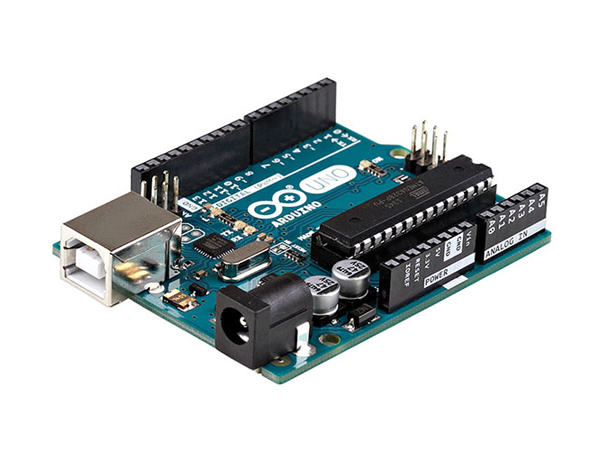
\includegraphics[scale=0.5]{arduino}
\end{center}
\subsection{NFC Shield v2.0}
Le shield sono schede che possono vengono inserite sopra l'Arduino, permettono l'estensione delle capacità della scheda stessa.La shield usata un questo progetto è quella NFC composta da un'antenna che collegandosi ad Arduino abilita la capacità di leggere/scrivere sui chip NFC
\begin{center}
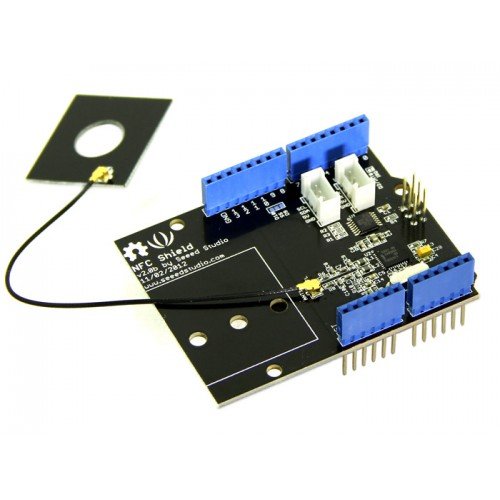
\includegraphics[scale=0.5]{shield}
\end{center}
\subsection{NFC Tag}
La tecnologia NFC  è una combinazione d'identificazione senza contatto (\textbf{RFID}) e altre tecnologie di connettività.NFC permette una comunicazione bidirezionale: quando due apparecchi NFC (initiator e target) vengono accostati entro un raggio di 4 cm, viene creata una rete peer-to-peer tra i due ed entrambi possono inviare e ricevere informazioni.
\\La tecnologia NFC opera alla frequenza di 13,56 MHz e può raggiungere una velocità di trasmissione massima di 424 kbit/s.
\\Il formato dei chip NFC usato nel progetto è \textbf{NDEF} [SPIEGAZIONE NDEF ?]
\subsection{Java}
Java è un linguaggio di programmazione ad alto livello, orientato agli oggetti e a tipizzazione statica, specificamente progettato per essere il più possibile indipendente dalla piattaforma hardware di esecuzione (tramite compilazione in bytecode prima e interpretazione poi da parte di una JVM), la scelta di questo linguaggio è dovuta alla politica \textbf{WORA} ovvero Write Once, Run Anywhere. Infatti il risultato dell'elaborato è un file con estensione \textit{JAR} il quale rende possibile l'uso su ogni dispositivo a patto che abbia installato java
\subsection{NoSQL Database}
NoSQL è una tecnologia che promuove sistemi software dove la persistenza dei dati è in generale caratterizzata dal fatto di non utilizzare il modello relazionale. L'espressione "NoSQL" fa riferimento al linguaggio SQL, che è il più comune linguaggio di interrogazione dei dati nei database relazionali.
\\Questi archivi di dati il più delle volte non richiedono uno schema fisso (schemaless), evitano spesso le operazioni di giunzione (join) e puntano a scalare in modo orizzontale. Gli accademici e gli articoli si riferiscono a queste basi di dati come memorizzazione strutturata (structured storage). Per il progetto è stata utilizzata questa tecnologia per tenere in memoria fisica (tramite un file con estensione .txt) gli abbonamenti dei vari utenti
\newpage
\thispagestyle{plain} % empty
\mbox{}
%\section{Tecnologia Implementata}
In questa sezione verranno illustrate le tecnologie implementate per la realizzazione del progetto
\subsection{NDEF e Sicurezza}
NDEF è un preciso standard per un formato di dati sui chip NFC, viene utilizzato in applicazioni quali le carde di credito, o gli smart poster, la struttura di un messaggio è quella vista nella seguente figura: 
\begin{center}
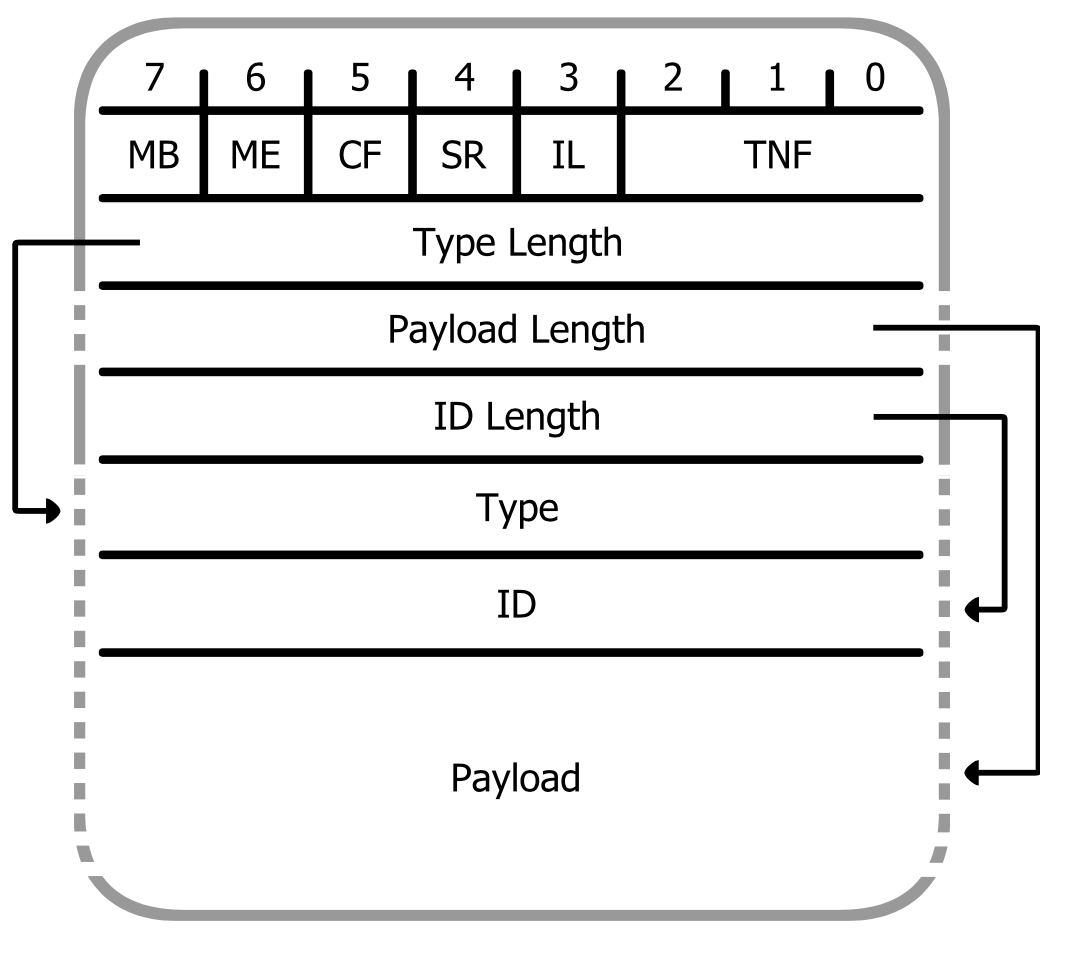
\includegraphics[scale=0.45]{ndefstructure}
\end{center}
In ordine abbiamo: 
\paragraph{Header}
\subparagraph{•}Message Begin (MB)
\subparagraph{•}Message End (ME)
\subparagraph{•}Chunk Flag (CF)
\subparagraph{•}Short record (SR)
\subparagraph{•}ID Length present (IL)
\subparagraph{•}Type Name Format (TNF)
\subparagraph{•}Length fields
\subparagraph{•}Type
\subparagraph{•}ID
\\I primi 5 parametri sono dei Flag, per finire invece abbiamo il \textbf{Payload} che è il messaggio.
\\Detto questo andiamo a concentrarci meglio su determinati campi quindi:
\paragraph{•}CF: indica il record che fa parte di una catena di record, quando il suo valore è pari a 1 vuol dire che c'è \textit{almeno} 1 altro record nella catena, invece quando non è settato vuol dire che ci troviamo o nel caso di record singolo o nel caso di ultimo elemento della catena. Una cosa da notare è che ME e CF non possono essere entrambi settati a 1
\paragraph{•}SR: quando viene messo ad 1 vuol dire che il record corrente è di tipologia short, questo comporta che il campo Payload Length, che si trova dentro Length fields, viene espresso tramite 1 byte, in alternativa viene espresso da 4 byte
\paragraph{•} IL: indica se nel record è presente un identificatore, se non dovesse essere abilitato questo comporta che non vi saranno il campo ID Length e il campo ID che è quello di identificazione del record.
\paragraph{•}TNF: serve per indicare la struttura del campo Type, è composto da 3 bit e può assumere solo i valori da 0 a 6 perché il numero 7 è riservato.
\\\\NDEF ha anche una firma
\begin{center}
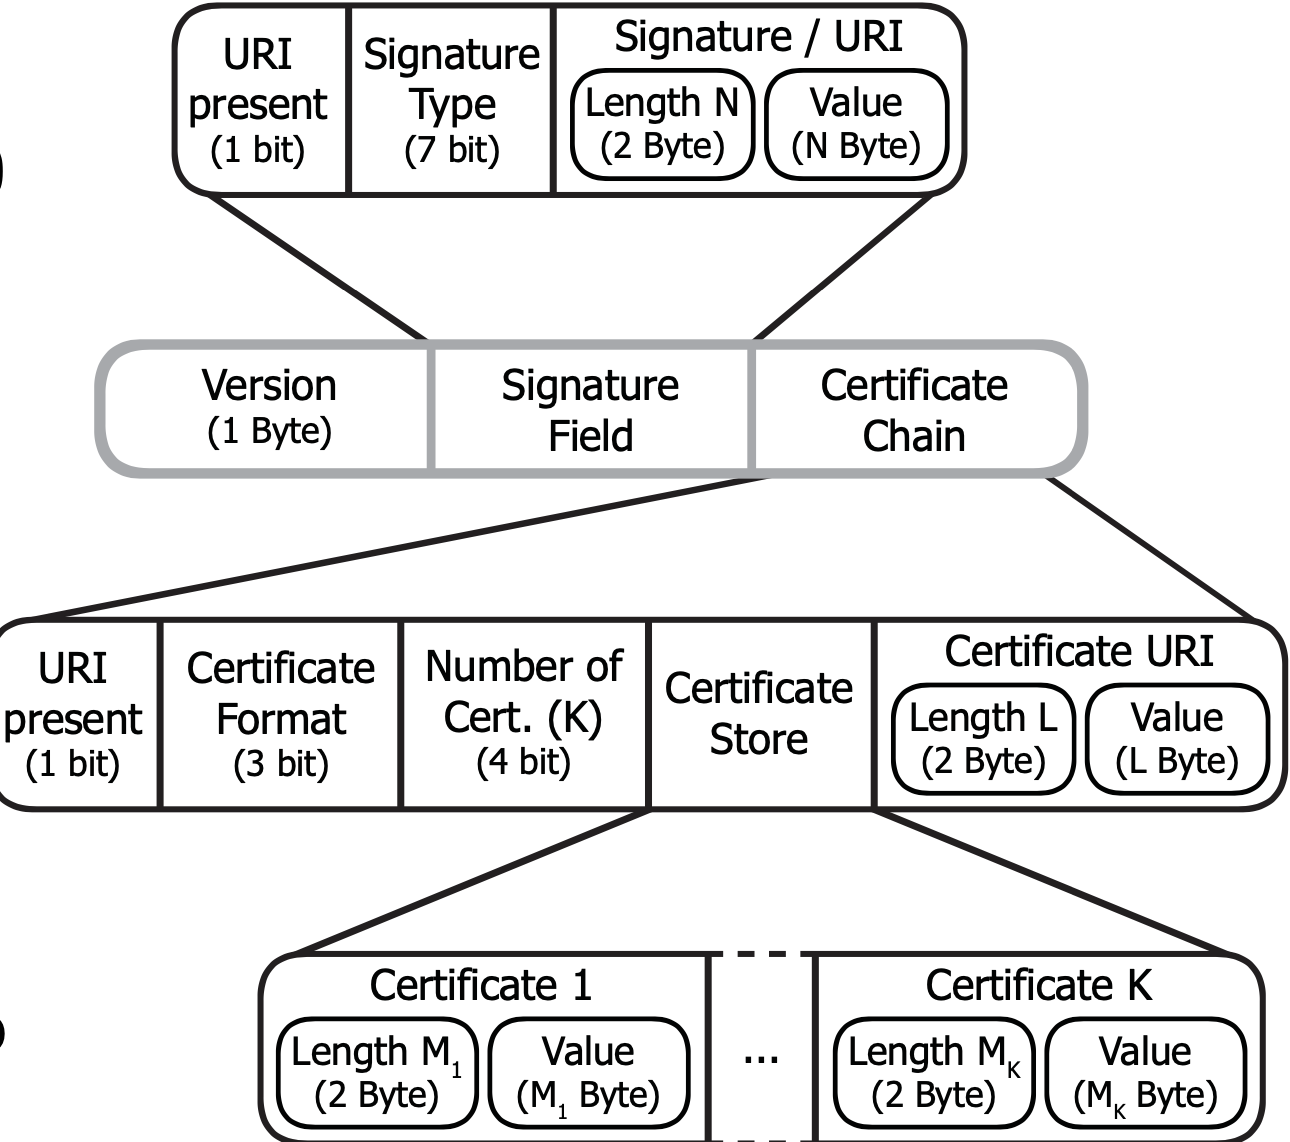
\includegraphics[scale=0.45]{ndefsign}
\end{center}
L'ultimo documento di specifica è stato rilasciato nel Novembre 2010, sostanzialmente ha una struttura fatta da un \textbf{campo firma}, che può essere una firma o una referenza URI ad una firma e da una \textbf{catena di certificati}, che è una catena di certificati PKI su un percorso sicuro.
\\Il record con la firma viene aggiunto ad una sequenza di record, e questo firma ogni record tra il record di firma appena precedente e se stesso, infatti un messaggio NDEF può contenere più di una firma.
\subsubsection{Cosa viene firmato?}
I campi che non vengono firmati sono MB/ME, questo perché se venissero firmati la firma non potrebbe essere agganciata al messaggio NDEF già firmato. Type, ID e Payload invece vanno firmati per assicurare l'integrità dei dati, mentre quando TNF viene cambiato, l'intero significato del record cambia, può essere quindi usato per nascondere dei record (identificati da type "Unknown"). 
\subsubsection{Sicurezza}
La tecnologia NFC è un'evoluzione dell'RFID, da un lato risulta meno predisposta ad attacchi esterni ma dall'altro lato è soggetta alle problematiche di sicurezza del suo predecessore. Le possibili minacce di sicurezza a cui sono sottoposti sono quelle riguardanti l'acquisizione, o l'alterazione dei dati contenuti nel tag, queste minacce possono avvenire mediante interrogazioni fraudolente o mediante intercettazione delle informazioni grazie a ricevitori radio durante la lettura da parte di un lettore autorizzato.
\subsubsection{Intercettazioni}
da fare
\subsubsection{Modifica dei dati}
da fare
\subsubsection{Man in the middle}
da fare
\subsection{Inserimento di falsi messaggi}
da fare
\subsection{NoSQL Database}
NoSQL è una tecnologia che promuove sistemi software dove la persistenza dei dati è in generale caratterizzata dal fatto di non utilizzare il modello relazionale. L'espressione "NoSQL" fa riferimento al linguaggio SQL, che è il più comune linguaggio di interrogazione dei dati nei database relazionali.
\\Questi archivi di dati il più delle volte non richiedono uno schema fisso (schemaless), evitano spesso le operazioni di giunzione (join) e puntano a scalare in modo orizzontale. Gli accademici e gli articoli si riferiscono a queste basi di dati come memorizzazione strutturata (structured storage). Per il progetto è stata utilizzata questa tecnologia per tenere in memoria fisica (tramite un file con estensione .txt) gli abbonamenti dei vari utenti
\subsection{WindowBuilder}
Per la realizzazione dell'interfaccia grafica in Java è stato usato il plug-in WIndowBuilder di Eclipse. Questo plug-in è composto a partire dalle liberire SWT Designer e Swing Designer e rende comoda e veloce la creazione di interfacce grafiche (GUI) per le applicazioni Java. Usando il WYSIWYG visual designer e gli strumenti di layout è possibile creare finestre complesse, e per ogni elemento messo verrà generato il codice contente la posizione dell'elemento e la sua dichiarazione.
\\Inoltre, il codice generato da questa libreria non richiede l'uso di altre librerie personalizzate per compilarlo ed eseguirlo, inoltre è possibile dall'interfaccia grafica creare eventi che poi andranno compilati mediante codice scritto in dei blocchi di \textit{ActionListener}, è possibile generare diversi tipi di eventi, dal click del mouse, alla pressione di un tasto sulla tastiera, o persino al movimento nella finestra del mouse.

\subsection{Cassandra}
Apache Cassandra è un DBMS distribuito e open source. Si tratta di un progetto Top-Level, sviluppato da Apache Software Foundation per gestire grandi quantità di dati dislocati in diversi server, fornendo un servizio orientato alla disponibilità.
\\È una soluzione NoSQL che inizialmente fu sviluppata da Facebook, un modello di dati simile a BigTable in esecuzione su un'infrastruttura tipi Amazon-Dynamo. Cassandra fornisce una struttura di memorizzazione chiave-valore, con Eventual Consistency.
\begin{center}

\includegraphics[scale=0.15]{cassandra}
\end{center}
Alle chiavi corrispondono dei valori, raggruppati in famiglie di colonne: una famiglia di colonne è definita quando il database viene creato. Tuttavia le colonne possono essere aggiunte a una famiglia in qualsiasi momento.
\\Le colonne sono aggiunte solo specificando le chiavi, così differenti chiavi possono avere differenti numeri di colonne in una data famiglia. I valori di una famiglia di colonne sono memorizzati insieme, questo perché Cassandra adotta un approccio ibrido tra DBMS orientato alle colonne e la memorizzazione orientata alle righe.
\\Come caratteristiche principali abbiamo:
\paragraph{•} Decentralizzazione: i nodi nel cluster sono identici, non c'è alcun single point of failure
\paragraph{•} Fault-tolerance: i dati vengono replicati in maniera automatica su più nodi, la replica è supportata tramite vari data center e la sostituzione dei nodi può avvenire senza downtime.
\paragraph{•} Tunable consistency: il livello di coerenza può essere modificato (da writes never fail a block for all replicas to be readable).
\paragraph{•} Elasticità: il throughput di lettura o scrittura scala linearmente con l'aggiunta di nuove macchine, senza downtime e senza interruzione di alcun applicativo.

\subsection{UUID}
\subsection{Crittografia}
%\newpage
%\thispagestyle{plain} % empty
%\mbox{}
\section{Implementazione}
\definecolor{codegreen}{rgb}{0,0.6,0}
\definecolor{codegray}{rgb}{0.5,0.5,0.5}
\definecolor{codepurple}{rgb}{0.58,0,0.82}
\definecolor{backcolour}{rgb}{0.95,0.95,0.92}

\hspace{\parindent}In questa sezione verranno illustrate le tecnologie utilizzate per la realizzazione dell'elaborato e verranno commentati dei tratti di codice fondamentali
\subsection{NDEF e Sicurezza}
\hspace{\parindent}NDEF è un preciso standard per un formato di dati sui chip NFC, viene utilizzato in applicazioni quali le carde di credito, o gli smart poster, la struttura di un messaggio è quella vista nella seguente figura: 
\begin{figure}[h]
\begin{center}
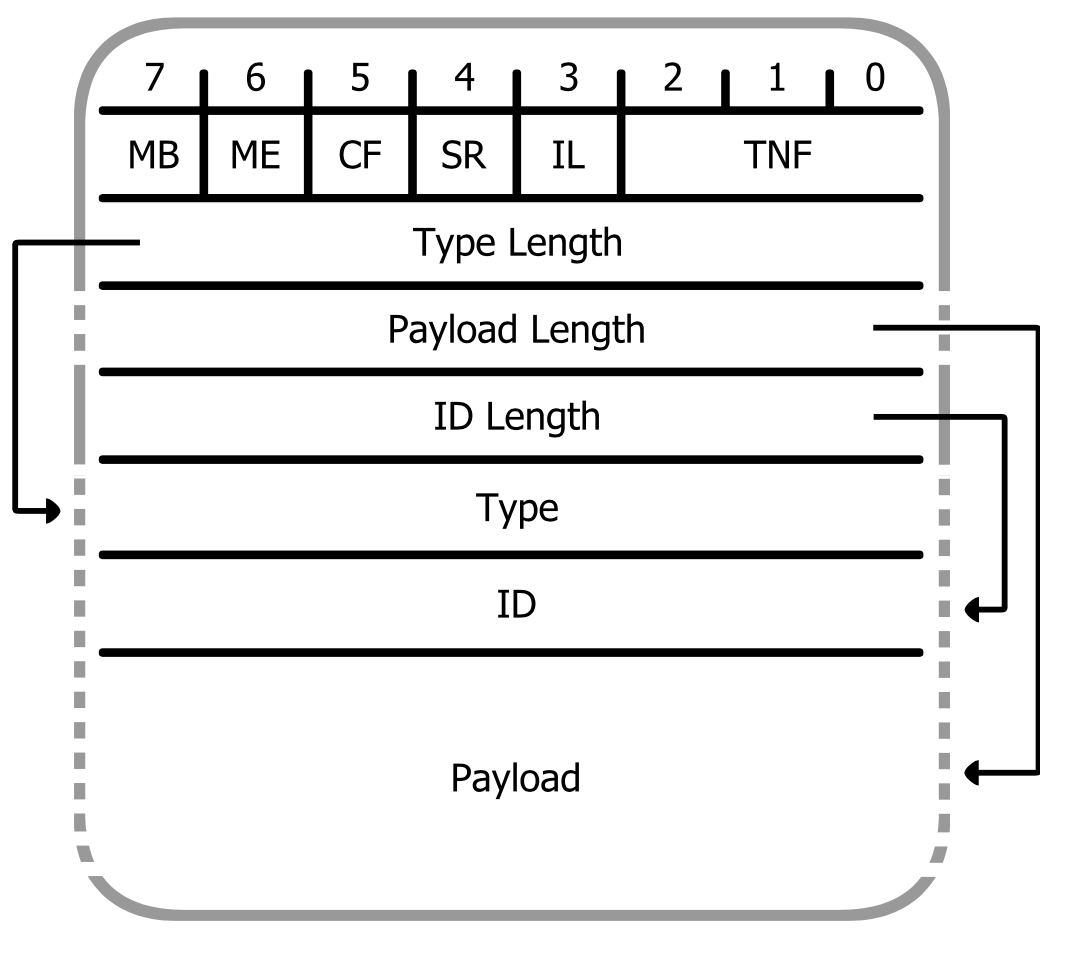
\includegraphics[scale=0.45]{ndefstructure}
\caption[NDEF Vulnerabilità]{Vulnerabilità NDEF\footnotemark}
\end{center}
\end{figure}
\footnotetext{\url{www.researchgate.net/publication/224227216_Security_Vulnerabilities_of_the_NDEF_Signature_Record_Type}}
In ordine abbiamo: 
\paragraph{Header}
Che è composto da: Message Begin (MB), Message End (ME), Chunk Flag (CF), Short record (SR), ID Length present (IL), Type Name Format (TNF), Length fields, Type, ID
\\I primi 5 parametri sono dei flag, per finire invece abbiamo il \textbf{Payload} che è il messaggio.
\\Detto questo andiamo a concentrarci meglio su determinati campi quindi:
\paragraph{•}CF: indica il record che fa parte di una catena di record, quando il suo valore è pari a 1 vuol dire che c'è \textit{almeno} 1 altro record nella catena, invece quando non è settato vuol dire che ci troviamo o nel caso di record singolo o nel caso di ultimo elemento della catena. Una cosa da notare è che ME e CF non possono essere entrambi settati a 1
\paragraph{•}SR: quando viene messo ad 1 vuol dire che il record corrente è di tipologia short, questo comporta che il campo Payload Length, che si trova dentro Length fields, viene espresso tramite 1 byte, in alternativa viene espresso da 4 byte
\paragraph{•} IL: indica se nel record è presente un identificatore, se non dovesse essere abilitato questo comporta che non vi saranno il campo ID Length e il campo ID che è quello di identificazione del record.
\paragraph{•}TNF: serve per indicare la struttura del campo Type, è composto da 3 bit e può assumere solo i valori da 0 a 6 perché il numero 7 è riservato.
\\\\NDEF ha anche una firma
\begin{figure}[h]
\begin{center}
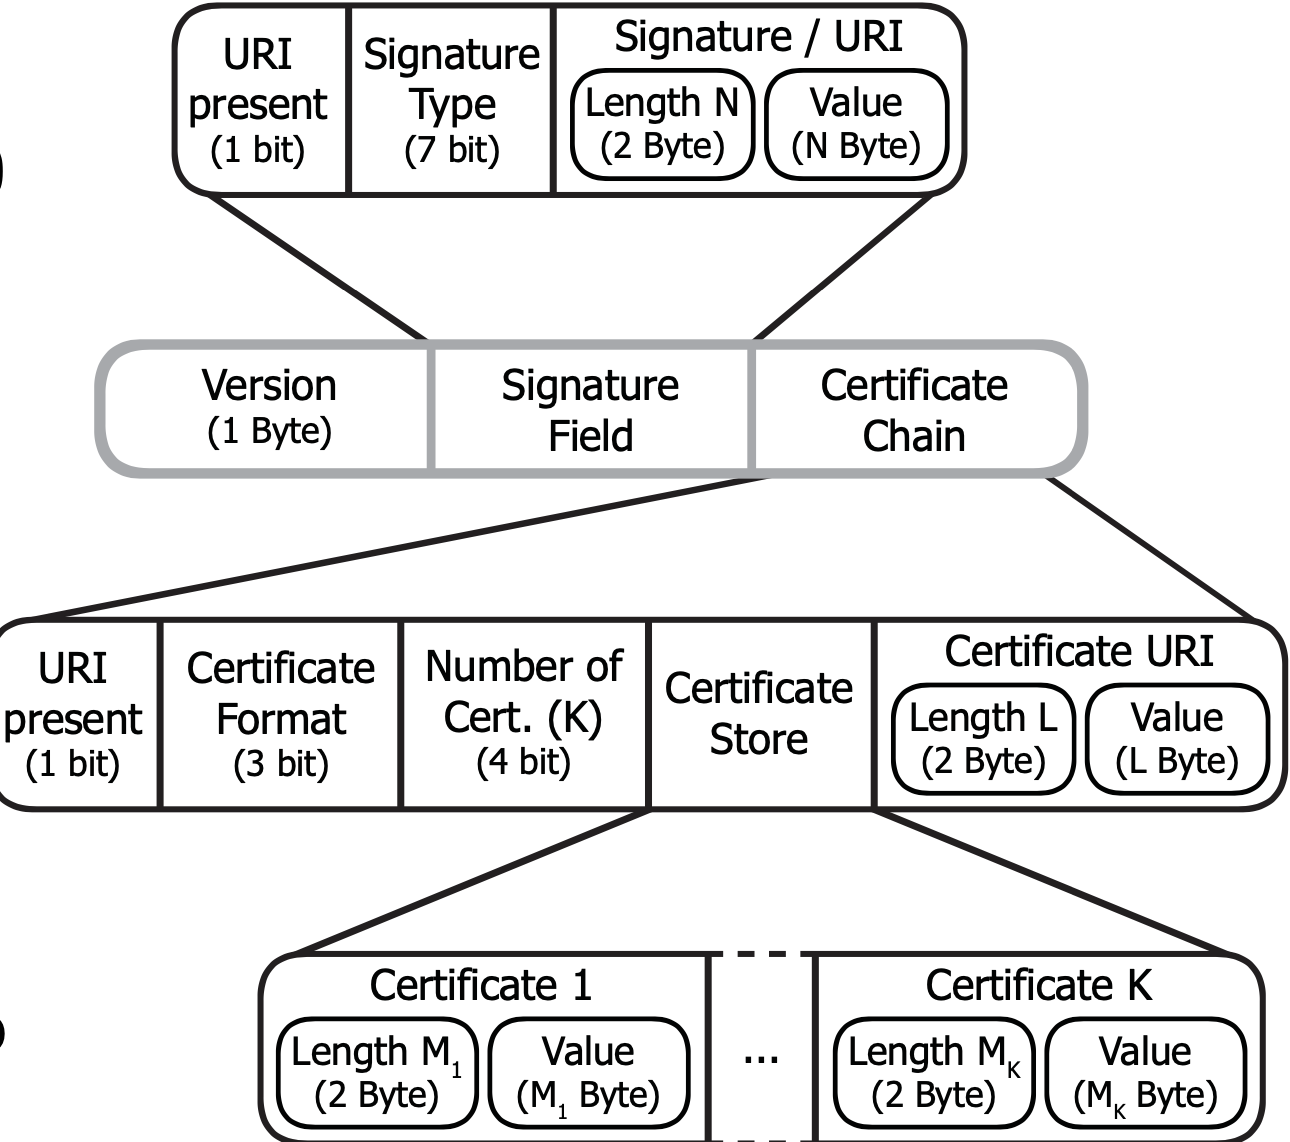
\includegraphics[scale=0.6]{ndefsign}
\caption[NDEF Vulnerabilità]{Vulnerabilità NDEF\footnotemark}
\end{center}
\end{figure}
\footnotetext{\url{www.researchgate.net/publication/224227216_Security_Vulnerabilities_of_the_NDEF_Signature_Record_Type}}
\\L'ultimo documento di specifica è stato rilasciato nel Novembre 2010, sostanzialmente ha una struttura fatta da un \textbf{campo firma}, che può essere una firma o una referenza URI ad una firma e da una \textbf{catena di certificati}, che è una catena di certificati PKI su un percorso sicuro.
\\Il record con la firma viene aggiunto ad una sequenza di record, e questo firma ogni record tra il record di firma appena precedente e se stesso, infatti un messaggio NDEF può contenere più di una firma.
\subsubsection{Cosa viene firmato?}
\hspace{\parindent} I campi che non vengono firmati sono MB/ME, questo perché se venissero firmati la firma non potrebbe essere agganciata al messaggio NDEF già firmato. Type, ID e Payload invece vanno firmati per assicurare l'integrità dei dati, mentre quando TNF viene cambiato, l'intero significato del record cambia, può essere quindi usato per nascondere dei record (identificati da type "Unknown"). 
\subsubsection{Sicurezza}
\hspace{\parindent}La tecnologia NFC è un'evoluzione dell'RFID, da un lato risulta meno predisposta ad attacchi esterni ma dall'altro lato è soggetta alle problematiche di sicurezza del suo predecessore. Le possibili minacce di sicurezza a cui sono sottoposti sono quelle riguardanti l'acquisizione, o l'alterazione dei dati contenuti nel tag, queste minacce possono avvenire mediante interrogazioni fraudolente o mediante l'intercettazione delle informazioni mediante ricevitori radio durante la lettura da parte di un lettore autorizzato.
\subsubsection{Intercettazioni}
\hspace{\parindent}Nell'ambito dell'NFC ma soprattutto in maniera generale, nel campo delle comunicazioni wireless l'intercettazione dei dati è uno degli attacchi più comuni. Per effettuare quest'attacco serve attrezzatura progettata ad hoc, quindi antenne e lettori fatti su misura. Per quanto riguarda il caso specifico NFC è un attacco molto difficile da realizzare a causa sei seguenti fattori:
\paragraph{i} potenza emessa dallo strumento sotto intercettazione
\paragraph{ii} fattori ambientali
\paragraph{iii} presenza della crittografia

Quindi da questo capiamo che anche in base al tipo di tag \footnote{cap 2 par 2.3.1} un attacco può essere più facile o più difficile, per esempio un attacco su un tag di tipo 1 sarà molto più semplice che su un tag di tipo 4.
\\Ci sono anche contromisure come per esempio quella di diminuire il campo magnetico, magari aumentando il fattore di direzionalità delle antenne, oppure usare algoritmi di cifratura per il messaggio, algoritmi per esempio AES.
\subsubsection{Modifica dei dati}
\hspace{\parindent}La modifica dei dati è un problema molto pericoloso, questo perché risulta trasparente all'utente, ha come scopo quello di modificare i dati trasmessi e renderli "validi". Fortunatamente risulta un attacco molto difficile da eseguire perché bisognerebbe riuscire ad intercettare completamente ogni bit del messaggio e rimandarlo sulle frequenze precise, quindi ogni volta modulando il campo delle frequenze in modo specifico e diverso.
\subsubsection{Man in the middle}
\hspace{\parindent}È uno degli attacchi più pericolosi, infatti può arrecare molti danni ai sistemi coinvolti. Mentre sysA e sysB stanno comunicando, sysH, il dispisitivo dell'hacker, si interpone tra di loro. Durante la comunicazione sysH altera il dialogo che hanno sysA e sysB, mettendosi in mezzo e fingendosi sysA per sysB e sysB per sysA. La soluzione a questo attacco è quella di instaurare un canale sicuro, quindi usando una chiave per criptare i dati. 
Potrebbe succede che sysH cerchi di negoziare una chiave ai due sistemi però è molto complesso perché richiederebbe la visibilità di sysH.

\subsection{UUID}
\hspace{\parindent}Un UUID\footnote{https://tools.ietf.org/html/rfc4122} conosciuto anche come Universally Unique Identifier, è un numero di 128 bit utilizzato per identificare informazioni nei sistemi informatici, lo si può trovare nell'rfc 4122.
\subsubsection{Come è formato?}
Il codice è composto da 16 byte, solitamente viene identificato da 32 caratteri esadecimali, a livello di sicurezza assume $ 3 \cdot 10^{38}$ possibili combinazioni
\begin{center}
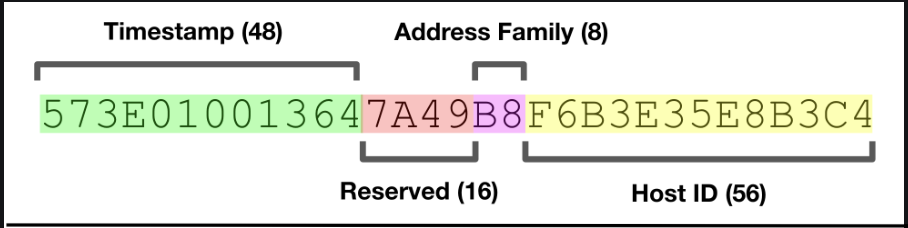
\includegraphics[scale=0.5]{uuid}
\end{center}
A differenza di altri sistemi l'unicità del codice generato non dipende da un'autorità centrale di registrazione o dal coordinamento delle parti che lo generano, però la sua probabilità di essere duplicato è talmente vicina a zero che viene considerata trascurabile.

\subsubsection{Analisi a livello matematico}

\hspace{\parindent}Considerando i 128 bit dell'UUID versione 4, 6 bit vengono riservati, quattro per la versione e due per altri parametri, quindi un UUID generato randomicamente ha 122 bit casuali. La probabilità che due UUID hanno lo stesso valore può essere calcolata usando la teoria delle probabilità (Paradosso del compleanno \footnote{https://betterexplained.com/articles/understanding-the-birthday-paradox/}). Usando quindi quest'approssimazione possiamo calcolare:
\begin{equation}
p(n) \approx 1- e^{-\frac{n^2}{2\cdot 2^x}}
\end{equation}
Notiamo quindi che quando il termine $ \frac{n^2}{2\cdot 2^x}$ è vicino allo zero, la probabilità può essere direttamente approssimata in questo modo:
\begin{equation}
p(n) \approx \frac{n^2}{2\cdot 2^x}
\end{equation}
Analizzandolo quindi in modo numerico potremo pensare che anche generando 1 miliardo di UUID ogni secondo per i prossimi 100 anni la probabilità di creare almeno un duplicato sarebbe circa del 50\%.

\subsection{Crittografia}

\subsection{Analisi del codice}
\hspace{\parindent}In questa sezione verranno mostrati i frammenti più importanti del codice
\lstdefinestyle{mystyle}{
    backgroundcolor=\color{backcolour},   
    commentstyle=\color{codegreen},
    keywordstyle=\color{magenta},
    numberstyle=\tiny\color{codegray},
    stringstyle=\color{codepurple},
    basicstyle=\ttfamily\footnotesize,
    breakatwhitespace=false,         
    breaklines=true,                 
    captionpos=b,                    
    keepspaces=true,                 
    numbers=left,                    
    numbersep=5pt,                  
    showspaces=false,                
    showstringspaces=false,
    showtabs=false,                  
    tabsize=2
}
\lstset{style=mystyle}
\subsubsection{Avvio del DB NoSQL}
\lstinputlisting[language=bash]{./Code/avvio.sh}

Automaticamente il controllore mettendo i suoi dati (validi) apre la connessione al database e va direttamente alla pagina di controllo degli abbonamenti
\subsubsection{Creazione del Database}
\lstinputlisting[language=bash]{./Code/CreazioneDB.sh}

La creazione del database viene fatta una sola volta, prima del rilascio dell'applicazione. 
\\Potrebbero succedere problemi hardware, oppure il link potrebbe perdere la connessione magari durante un processamento dei dati, per questo una soluzione è quella di avere un backup disponibile appena succede un problema, quindi i dati vengono replicati per assicurare che non ci siano fallimenti. Cassandra posiziona le repliche dei dati su nodi diversi in base a due fattori:
\paragraph{•} Strategia di replicazione
\paragraph{•} Fattore di replicazione
Il primo dice dove posizionare le replica, il secondo invece determina quante repliche vengono posizionate, un esempio lo troviamo nella riga 4 dove abbiamo la stringa \textit{'replication\_factor' : 3}, questo indica che vengono fatte 3 repliche su 3 nodi diversi. Solitamente per garantire che non ci siano fallimenti il fattore di replicazione deve essere 3.
\\Nella riga 3 vediamo la stringa \textit{'SimplyStrategy'}, questa viene usata quando abbiamo un solo data center, quindi la prima replica viene posizionata sul nodo selezionato dal partizionatore, dopo questo, le restanti repliche vengono posizionate in senso orario a partire dalla direzione del nodo.
\subsubsection{Creazione tabella DB}
\lstinputlisting[language=bash]{./Code/CreazioneTabella.sh}

Anche questa parte di codice, come la creazione del database viene fatta una sola volta, prima del lancio dell'applicazione
\subsubsection{Connnessione al database mediante CQLSH}
\subsubsection{Connessione al DB NoSQL}
\lstinputlisting[language=Java]{./Code/Connessione.java}

In questo frammento di codice viene mostrato il metodo con il quale viene fatta la connessione al database NoSQL Cassandra!
\subsubsection{Apertura della connessione con la porta seriale in Java}
\lstinputlisting[language=Java]{./Code/AperturaSeriale.java}

Nel frammento di codice appena visto c'è la dichiarazione delle porte che si vanno ad utilizzare, il \textbf{DATA\_RATE}, ovvero la quantità di dati digitali che possono essere trasferiti su un canale in un determinato intervallo temporale e l'apertura della connessione tramite la funzione \textbf{portId.open}
\subsubsection{Rilevamento presenza tag NFC Arduino}
\lstinputlisting[language=c++]{./Code/RilevamentoPresenze.cpp}

In questo frammento di codice viene evidenziato come il chip NFC se presente viene scannerizzato, l'unica cosa che verrà presa sarà il payload e non l'intestazione! Questo perché l'intestazione ci serve solo a sapere se il chip è formattato in formato NDEF
\subsubsection{Creazione abbonamento in Java}
\lstinputlisting[language=Java]{./Code/CreazioneAbbonamento.java}

Nella prima riga notiamo subito la variabile \textit{zoneatt}, in questa vi saranno le zone selezionate in precedenza per la creazione dell'abbonamento, nella riga numero 6 notiamo il comando importantissimo \textit{output.write(zoneatt)}, questo comando ci permette di scrivere sulla porta seriale le zone, che verranno successivamente codificate e poi scritte sul tag NFC.
\subsubsection{Scrittura abbonamento nel Database}
\lstinputlisting[language=Java]{./Code/ScritturaDB.java}

Le righe 5 e 6 servono per definire i parametri per la connessione, quindi indirizzo IP e porta, la linea 3 serve ad istanziare l'oggetto client che sarà quello che ci permetterà la connessione al database e la linea 9 ci permetterà l'apertura della connessione col database.
\\Andando avanti nel codice creiamo un abbonamento nel quale vengono passati i parametri da specifiche funzioni\footnote{i parametri sono presi dalla form di creazione dell'abbonamento e vengono crittografati}, per finire troviamo il comando più importante \textit{client.esegui()}, questo ci permetterà l'inserimento dei dati nel database, infatti eseguirà questo comando:
\begin{center}
\lstinputlisting[language=sql]{./Code/Query.sql.txt}
\end{center}
\subsubsection{Scrittura abbonamento su tag NFC }
\lstinputlisting[language=c++]{./Code/scritturaAbbonamento.cpp}


\newpage
\thispagestyle{plain} % empty
\mbox{}
%\include{./Chapters/Esfunzionamento}
\include{./Chapters/sviluppiFuturi}
\newpage
\thispagestyle{plain} % empty
\mbox{}
\section{Bibliografia}
\begin{enumerate}[label={[\arabic*]}]
\item ciao.
\item aoooo.
\end{enumerate}
%\include{./Chapters/Conclusione}

\end{document}
